\documentclass[a4paper,11pt]{article}

%%%%%%%%%%%%%%%%%%%%%%%%%%%%%%%%%%%%%%%%%%%%%%%%%%%%%%%%%%%%%%%%%%%%%%%%%
\pagestyle{plain}                                                      %%
%%%%%%%%%% EXACT 1in MARGINS %%%%%%%                                   %%
\setlength{\textwidth}{6.6in}     %%                                   %%
\setlength{\oddsidemargin}{-0.06in}   %% (It is recommended that you       %%
\setlength{\evensidemargin}{-0.06in}  %%  not change these parameters,     %%
\setlength{\textheight}{9.1in}    %%  at the risk of having your       %%
\setlength{\topmargin}{0in}       %%  proposal dismissed on the basis  %%
\setlength{\headheight}{-0.1in}      %%  of incorrect formatting!!!)      %%
\setlength{\headsep}{0in}         %%                                   %%
%\setlength{\footskip}{.5in}       %%                                   %%
%%%%%%%%%%%%%%%%%%%%%%%%%%%%%%%%%%%%       
%%%%%%%%%%%%%%%%%%%%%%%%%%%%%%%%%%%%%%%%%%%%%%%%%%%%%%%%%%%%%%%%%%%%%%%%%
 \linespread{1.3}
\usepackage[dvips]{graphicx}
\usepackage{amsmath,bm}
\usepackage{amssymb}
\usepackage{psfrag}
\usepackage{hyperref}
\usepackage{color}
%\usepackage{subfigure}
\usepackage{bigfoot}
\usepackage{framed}
\usepackage{subcaption}
\usepackage{graphicx}

\usepackage[normalem]{ulem}


\newcommand{\bs}{\boldsymbol}
\def\RR{ \mathbb R}
\newcommand{\refeq}[1]{Equation \eqref{#1}}
\def\bl{ \mathbf \lambda}
\def\ba{ \beta}
%%%%%%%%%%%%%%%%%%%%%%%%%%%%%%%%%%%%%
\newcommand{\boxeq}[1]{%
  \[\fbox{%
      \addtolength{\linewidth}{-2\fboxsep}%
      \addtolength{\linewidth}{-2\fboxrule}%
      \begin{minipage}{\linewidth}%
      \begin{equation}#1\end{equation}%
      \end{minipage}%
    }\]%
}
%%%%%%%%%%%%%%%%%%%%%%%%%%%%%%%%%%%%%%%%%%%%%%%%%%%%%%%
\newcommand{\ee}{\end{equation}}
\newcommand{\be}{\begin{equation}}
\newcommand{\ec}{\end{center}}
\newcommand{\bc}{\begin{center}}
\newcommand{\eea}{\end{eqnarray}}
\newcommand{\bea}{\begin{eqnarray}}
\newcommand{\bd}{\begin{description}}
\newcommand{\ed}{\end{description}}
\newcommand{\bi}{\begin{itemize}}
\newcommand{\ei}{\end{itemize}}
\newcommand{\pa}{\partial}

\newcommand{\bx}{\bs{x}}
\newcommand{\bxi}{\bx^{(i)}}
\newcommand{\bxn}{\bx^{(n)}}

\newcommand{\by}{\bs{y}}
\newcommand{\byn}{\by^{(n)}}

\newcommand{\br}{\bs{r}} 
\newcommand{\brn}{\bs{r}^{(n)}} 

\newcommand{\bz}{\bs{z}}

	\newcommand{\pt}{p^{trans}}



\newcommand{\bxx}{\bs{X}}
\newcommand{\bxb}{\bar{\bs{X}}}
\newcommand{\byy}{\bs{Y}}

\newcommand{\bt}{\bs{\theta}}
\newcommand{\btt}{\bs{\Theta}}


\newcommand{\bp}{\bs{\phi}}

\newcommand{\beps}{\bs{\epsilon}}
\newcommand{\qe}{q_{\epsilon}(\bs{\epsilon})}

\newcommand{\bax}{\bs{A}_x}
\newcommand{\bbx}{\bs{b}_x}
\newcommand{\bvx}{\bs{V}_x}
\newcommand{\bcx}{\bs{C}_x}
\newcommand{\bdx}{\bs{D}_x}
\newcommand{\E}{\mathbb{E}}





\title{Stochastic optimization Module : Application to concrete column simulation}
\author{Atul Agrawal}
%\date{\today}

\begin{document}

\maketitle




Notation:
\bi
\item $\bx$: concrete mix parameters (also optimization variables ultimately)
\item $\bs{b}$: hydration model input parameters
\item $\by_c$ or $\by_c(\bs{b})$ : hydration model output(s) relevant for calibration
\item $\by_o$ or $\by_o(\bs{b})$ : hydration model  output(s) relevant for optimization (e.g. KPIs)
\ei
Suppose $N$ data-pairs $\mathcal{D}_N$  are available which consist of $\mathcal{D}_N=\{ \hat{\bx}^{(i)},  \hat{\by}_c^{(i)}\}_{i=1}^N$. We would like to use those to infer the corresponding $\bs{b}^{(i)}$ but more importantly the relation between $\bx$ and $\bs{b}$ (performed in the calibration module)  which would be of relevance for downstream, optimization tasks.






\section{Optimization}

The task of optimization can be summarized as finding the optimum concrete mix parameters $\bm x \in \RR$ (e.g, cement type ratio) in order to minimize certain (stochastic) objective such that a stochastic inequality constraints are satisfied. Consider the following for the current formulation:

\begin{align}
	&\min_{\bm x} \mathcal{O}(\bm x)= \E_{\bm b\sim p(\bm b | \bm x, \bm {\varphi}^*)}[y_{o}(\bm b)]\\
	&\text{s.t} ~~ \E_{\bm b\sim p(\bm b | \bm x, \bm {\varphi}^*)}[y_{c_i}(\bm b)] \leq \alpha_i, \quad i = 1,\cdots, m
\end{align}

Here, $\bm{\varphi}^*$ denotes the learnt parameters between  $\bm b$ and $\bm x$, $y_{o}$ denotes the solver output corresponding to the objective and $y_{c_i}$ the solver output corresponding to the $i^{th}$ constraint. 
%Simplifying the notations a bit further, lets say $\mathcal{O}(\bm x)$ denotes the objective and $\mathcal{C}_{i}(\bm x)$ denotes the $i^{th}$ constraint.
The problem can be approached with penalty-based methods
\footnote{ \href{https://web.stanford.edu/class/ee364a/lectures/stoch\_prog.pdf}{https://web.stanford.edu/class/ee364a/lectures/stoch\_prog.pdf} } \cite{wang_stochastic_2003}  by defining the following objective:

\begin{align}
	\min_{\bm x} \mathcal{O}(\bm x) + \sum_{i=1}^{m}c_i \mathcal{C}_i(\bm x)
\end{align}
where $c_i>0$ are penalty parameters for violating constraints and $\mathcal{C}_{i}(\bm x) = \max (\E_{\bm b\sim p(\bm b | \bm x, \bm {\varphi}^*)}[y_{c_i}(\bm b)] - \alpha_i,0)$. Alternatively, the problem can also  be approached with the Augmented Lagrangian Method \footnote{\href{https://www.him.uni-bonn.de/fileadmin/him/Section6\_HIM\_v1.pdf}{https://www.him.uni-bonn.de/fileadmin/him/Section6\_HIM\_v1.pdf}}

To test the scheme, a concrete column simulation with the hydration model is formulated \cite{} (@Erik can add the description if need be) for which the objective (Key performance Indicator (KPI)) is the critical time ($t_c$) at which the max yield is reached and there is a single constraint pertaining to the expected  max. temperature ($T$). % at no point in time should increase a certain value. 
Following the notations above, we have:

\begin{align}
&\min_{\bm x} \mathcal{O}(\bm x)= \E_{\bm b\sim p(\bm b | \bm x, \bm {\varphi}^*)}[t_c(\bm b)]\\
&\text{s.t} ~~ \E_{\bm b\sim p(\bm b | \bm x, \bm {\varphi}^*)}[T(\bm b)] \leq \alpha
\end{align}

The problem is solved using the  penalty-based objective described above and score function gradient estimators \cite{schulman_gradient_2016} are used to compute the expectation gradients. The implementation is performed in PyTorch library.
Some initial results are depicted in Fig. \ref{fig:opt_diagnostics_hydration} for $\alpha = 68^o$. As can be seen from the Fig. \ref{fig:para_opt_hydration}, the constraints started to be violated close to $\bm x \sim 0.6$ which led to negative gradients, which reversed the descend of the optimization parameter (by observation $\mathbb{E}[T] \propto 1/\bm{x}$ and $\mathbb{E}[t_c] \propto \bm{x}$) and stabilized it to a value which also satisfies the constraints.

\begin{figure}[!htpb]
	\centering
	\begin{subfigure}{0.45\textwidth}
		\includegraphics[width=\textwidth]{fig/X_evolution_opt_2022_10_27-11_09_09_AM.pdf}
		\caption{Evolution of the Optimization variable $x$}
		\label{fig:para_opt_hydration}
	\end{subfigure}
	\hfill
	\begin{subfigure}{0.45\textwidth}
		\includegraphics[width=\textwidth]{fig/x_grad_evolution_opt_2022_10_27-11_09_09_AM.pdf}
		\caption{Monte Carlo estimated gradients}
		\label{fig:grad_opt_hydration}
	\end{subfigure}
	\hfill
	\begin{subfigure}{0.45\textwidth}
		\includegraphics[width=\textwidth]{fig/objective_opt_2022_10_27-11_09_09_AM.pdf}
		\caption{Evolution of the objective $\mathcal{O}(\bm x)$}
		\label{fig:objective_evolution}
	\end{subfigure}
	\hfill
	\begin{subfigure}{0.45\textwidth}
		\includegraphics[width=\textwidth]{fig/constraints_opt_2022_10_27-11_09_09_AM.pdf}
		\caption{Evolution of the temp. constraint $\mathcal{C}(\bm x)$}
		\label{fig:constraint_evolution}
	\end{subfigure}
	\hfill
	\caption{Optimization under uncertainty for concrete column with hydration model}
	\label{fig:opt_diagnostics_hydration}
\end{figure}
%\psk{The plots should include the evolution of the objective, the evolution of the constraint}
%\psk{what is the value of the penalty parameter, how  was it adapted, when and why did u stop increasing it. Formally these should be infinite.}
%\psk{What is the distribution of $t_c$ at the optimal $x$ incl. a clear demarcation of its mean which appears in the objective}
%\psk{What is the distribution of $T$ at the optimal $x$ incl. a clear demarcation of its mean which appears in the constraint}


 It is crucial to mention that computational cost of the forward solver can be a limiting factor in the optimization process. Efficient \textit{offline} surrogates can be developed for that. It can serve two purposes: i) Alleviate the computational bottleneck, ii) Potentially reduce the estimated variance of the gradients since the reparametrization trick can be used when  the surrogate is differentiable. 
 
 
The workflow of the stochastic optimization process is summarized in the Fig. \ref{fig:stochastic_opt_flowchart}. The stochastic optimization of the concrete column simulation just serves as a proof of concept and in theory the workflow should not be altered for change in the physics based model, objective function, constraints function etc. After the relationship between the mix parameters $\bm x$ and the latents (solver inputs $\bm b$) is inferred in the calibration module (if an analytic relation is not existing), the following \emph{links} are necessary to perform the optimization:
\begin{itemize}
	\item A physics based model $\bm y(\cdot)$ relating the inputs $\bm b$ and the outputs $y_o, y_{c_i}$.
	\item If possible, a surrogate of the model linking the inputs and the outputs.
	\item Clearly defined objective and the constraints. 
\end{itemize} 

 
 
 \begin{figure}[!htpb]
 	\centering
 	\includegraphics[width=0.8\textwidth]{fig/Optimisation_flowchart.pdf}
 	\caption{\emph{Stochastic optimisation workflow} : Circular nodes represents the stochastic nodes and the square represents the deterministic nodes.}
 	\label{fig:stochastic_opt_flowchart}
 \end{figure}
 



% adding Bib
\newpage
\nocite{*}
\bibliographystyle{unsrt}
%\bibliographystyle{abbrv}
\footnotesize{\bibliography{bibliography.bib}}
\end{document}


